%%
%% UnBTeX: A class for bachelor, master, and doctoral thesis at the
%% University of Brasilia (UnB), Brazil
%% Version 1.5.5 2025/04/10
%% Copyright (C) 2021-2025 by Henrique C. Ferreira <hcferreira@unb.br>
%%
%% This class file may be distributed and/or modified under the conditions
%% of the LaTeX Project Public License, either version 1.3 of this license
%% or (at your option) any later version. The latest version of this
%% license is in:
%% 
%%    https://www.latex-project.org/lppl.txt
%% 
%% and version 1.3 or later is part of all distributions of LaTeX version
%% 2005/12/01 or later.
%%
%% This file is a template for use with the UnBTeX class
%% To compile the document you should call pdflatex, bibtex, pdflatex
%% 

\documentclass[
    % -- Opção da classe memoir -- https://www.ctan.org/pkg/memoir
    oneside, % Para imprimir somente na frente da folha
    %twoside, % Para imprimir na frente e no verso da folha
    %draft, % Use para compilar pela primeira vez trabalhos com timeout
    % -- Opção da classe abntex2 -- https://www.ctan.org/pkg/abntex2
    sumario=tradicional, % Remova esta opção para sumário padrão ABNT
    % -- Selecione o idioma no qual o trabalho será escrito
    idioma=brazil, % Para texto principal em português
    %idioma=english, % Para texto principal em inglês  
    % -- Opções para as referências bibliográficas
    bib=alf, % Bibliografia nas normas da ABNT, estilo autor-data
    %bib=num, % Bibliografia nas normas da ABNT, estilo numérico
    refback, % Indica na bibliografia onde cada referência é citada
    % -- Selecione o estilo de numeração de figuras, tabelas, etc.
    numb=chap, % Numeração por capítulo
    %numb=abnt, % Numeração para o documento inteiro
    ]{unbtex}

% ---
% Pacotes básicos (Adicione outros pacotes necessários para o seu trabalho)
% ---
\usepackage{lscape} % Pacote para rotacionar tabelas (e outros objetos)
%\usepackage{pdflscape} % Pacote para rotacionar objetos e também a página do arquivo pdf
\usepackage{afterpage} % Evita quebra de página quando inserir uma tabela (ou outro objeto) rotacionada
% ---

% ---
% Compila a nomenclatura
% ---
\makenomenclature
% ---

% ---
% Diretório das figuras
\graphicspath{{unbtex-example/figuras}}
% --- 

% ------------------------------------------------------------------------
% ------------------------------------------------------------------------
% Informações do trabalho
% ------------------------------------------------------------------------
% ------------------------------------------------------------------------

% ---
% Título
% ---
\titulo{Modelo de trabalho\\ acadêmico com UnB\TeX} % No idioma principal do texto
% Insira \\ caso queira forçar quebras de linha no título
% Não utilize caixa alta para o título do trabalho e nem das seções (com exceção de siglas)
% ---
\tituloestrangeiro{} % Escreva aqui título em português se o trabalho for escrito em inglês (caso contrário, deixe vazio)
% ---

% ---
% Autores
% ---
\autori[]{Carlos}{Lisboa} % \autori[]{Nome}{Sobrenome}
% No caso de nomes como Carlos de Souza, utilize \autori[]{Carlos de}{Souza} (e não \autori[]{Carlos}{de Souza})
% ---
\autorii[]{}{} % Deixe os argumentos vazios se não tiver segundo autor
% ---

% ---
% Código Cutter para a ficha catalográfica
% Gerado a partir da entrada <Sobrenome, Nome> (do primeiro autor) no site https://www.tabelacutter.com/
% ---
\numerocutter{} % Para não imprimir o código na ficha catalográfica, deixe o argumento vazio
%\numerocutter{769} % Prencher o argumento do comando apenas com os números gerados
% ---

% ---
% Orientadores
% ---
\orientador[Orientador]{Prof. Dr.}{Lourenço Nassib}{Chehab} % Para alterar o gênero, basta trocar Orientador por Orientadora
%\orientador[Orientadora]{Profa. Dra.}{Sylla Helena}{Ortegosa da Cunha}
% ---
\coorientador[Coorientador]{Prof. Dr.}{}{} % Deixe os argumentos para nome e sobrenome vazios se não tiver coorientador 
% ---

% ---
% Informações do curso
% ---
\tipotrabalho{Trabalho de Conclusão de Curso} % Dissertação de Mestrado; Tese de Doutorado (em português, mesmo que o trabalho seja em inglês)
%\tipotrabalho{Tese de Doutorado}
% ---
\tipocurso{Engenharia Elétrica} % Nome do curso de graduação ou do programa de pós-graduação, em português
%\tipocurso{Programa de Pós-Graduação em Engenharia Elétrica}
% ---
% Texto que aparece na folha de rosto e na folha de aprovação
\preambulo{Trabalho de Conclusão de Curso submetido como requisito parcial para obtenção do grau de Engenheiro Eletricista.} 
%\preambulo{Tese de Doutorado submetida ao Programa de Pós-Graduação em Engenharia Elétrica da Universidade de Brasília como parte dos requisitos necessários para obtenção do grau de Doutor.}
% Consulte a secretaria/coordenação do curso para saber o que deve ser escrito no preâmbulo. Use português mesmo que o trabalho seja em inglês.
% ---
% Informação adicional para ser impressa na folha de rosto
\publicacao{} % Deixe o argumento vazio caso não haja
%\publicacao{Publicação PPGEE 201/23} % Também imprime as informações do trabalho no topo da página da ficha catalográfica
% ---

% ---
% Instituição
% ---
%\instituicao[Universidade de Brasília]{Faculdade de Tecnologia}{} % Use português mesmo que o trabalho seja em inglês
\instituicao[Universidade de Brasília]{Faculdade de Tecnologia}{Departamento de Engenharia Elétrica} % Caso queira incluir o departamento da unidade acadêmica
% ---

% ---
% Local e data da defesa
% ---
\local{Brasília}
\dia{10}
\mes{abril}
\ano{2025}
% ---

% ---
% Membros da banca
% ---
\membrodabancai{Prof. Dr. Lourenço Nassib Chehab\\ UnB/FT/ENE} % Membro 1 - Geralmente é o orientador
\membrodabancaifuncao{Orientador} % Em português, mesmo que o trabalho seja em inglês.
\membrodabancaii{Prof. Dr. Sérgio Barroso de Assis Fonseca\\ UnB/FT/ENE} % Membro 2
\membrodabancaiifuncao{Examinador interno}
\membrodabancaiii{Prof. Dr. Nelson Ortegosa da Cunha\\ UnB/FT/ENE} % Membro 3
\membrodabancaiiifuncao{Examinador interno}
\membrodabancaiv{} % Deixe vazio se não tiver o quarto membro
\membrodabancaivfuncao{Examinador externo}
\membrodabancav{} % Deixe vazio se não tiver o quinto membro
\membrodabancavfuncao{Examinador externo}
% Comprimento da linha da assinatura (ajuste conforme necessidade)
\signlinewidth{9cm}
% ---

% ---
% Resumo em português
% ---
\begin{Resumo}
Este documento exemplifica a elaboração de trabalho acadêmico (trabalho de conclusão de curso, dissertação e tese) a partir da classe UnB\TeX, uma extensão da classe \abnTeX\ para a Universidade de Brasília (UnB). Além de apresentar comandos básico de \LaTeX\ para inclusão de equações, tabelas e figuras, o documento mostra como utilizar pacotes adotados pela classe UnB\TeX\ para gerar referências bibliográficas, listas símbolos, caixas para teoremas e algoritmos, dentre outros elementos úteis ou obrigatórios para trabalhos acadêmicos. Espera-se que este documento facilite o uso da classe UnB\TeX\ na elaboração de trabalhos de alta qualidade gráfica mesmo por usuários com pouca experiência em \LaTeX.
\end{Resumo}
% ---

% ---
% Resumo em inglês
% ---
\begin{Abstract}
This document demonstrates the preparation of academic works (such as final papers, dissertations, and theses) using the UnB\TeX\ class, an extension of the \abnTeX\ class developed for the University of Brasília (UnB). In addition to introducing basic \LaTeX\ commands for the inclusion of equations, tables, and figures, the document shows how to utilize packages integrated with the UnB\TeX\ class to generate bibliographic references, lists of symbols, and formatted boxes for theorems and algorithms, among other essential or useful elements for academic writing. The goal is to simplify the use of the UnB\TeX\ class, enabling even users with minimal \LaTeX\ experience to produce visually high-quality academic documents.
\end{Abstract}
% ---

% ---
% Palavras-chave (defina no mínimo 3 e no máximo 5)
% ---
\pchavei{palavra-chave 1}
\kwordi{keyword 1}
\pchaveii{palavra-chave 2}
\kwordii{keyword 2}
\pchaveiii{palavra-chave 3}
\kwordiii{keyword 3}
\pchaveiv{palavra-chave 4} % Deixe vazio se não tiver
\kwordiv{keyword 4} % Deixe vazio se não tiver
\pchavev{} % Deixe vazio se não tiver
\kwordv{} % Deixe vazio se não tiver
% ---

% ---
% Agradecimentos
% ---
% Idioma usado nos agradecimentos (pode ser em português, mesmo que o trabalho seja em inglês)
\idiomaagradecimentos{brazil}
%\idiomaagradecimentos{english}

\begin{otherlanguage*}{\acklang}

% Primeiro autor
\begin{AgradecimentosAutorI}
Agradecemos ao Dr. Lauro César Araujo e equipe que desenvolveram a classe \abnTeX\ para escrita de trabalhos acadêmicos condizentes as normas da ABNT. A classe UnB\TeX\ a toma como base para atender necessidades específicas de cursos de graduação e pós-graduação da Universidade de Brasília.

Agradecemos também ao Prof. Dr. Leonardo Luiz e Castro pelo modelo em \LaTeX\ para livro para editora UnB, que teve alguns recursos adaptados para o UnB\TeX.
\end{AgradecimentosAutorI}

% Segundo autor
\begin{AgradecimentosAutorII}
Agradecimentos do segundo autor.
\end{AgradecimentosAutorII}

\end{otherlanguage*}
% ---

% ---
% Dedicatória
% ---

% Primeiro autor
\begin{DedicatoriaAutorI}
Este trabalho é dedicado às crianças adultas que,\\
quando pequenas, sonharam em se tornar cientistas.
\end{DedicatoriaAutorI}

% Segundo autor
\begin{DedicatoriaAutorII}
Dedicatória do segundo autor.
\end{DedicatoriaAutorII}
% ---

% ---
% Epígrafe
% ---
\begin{Epigrafe}
\vspace*{\fill}
\begin{flushright}
    \textit{``If you find that you're spending almost all your time on theory,\\
    start turning some attention to practical things;\\
    it will improve your theories.\\
    If you find that you're spending almost all your time on practice,\\
    start turning some attention to theoretical things;\\
    it will improve your practice.''\\
    (Donald Knuth)}
\end{flushright}
\end{Epigrafe}
% ---

% ------------------------------------------------------------------------
% ------------------------------------------------------------------------
% Início do documento
% ------------------------------------------------------------------------
% ------------------------------------------------------------------------
\begin{document}

% ------------------------------------------------------------------------
% ELEMENTOS PRÉ-TEXTUAIS
% ------------------------------------------------------------------------
\pretextual
% ------------------------------------------------------------------------

% Insere capa e contracapa
\imprimircapa

% Insere folha de rosto
\imprimirfolhaderosto*

% Insere ficha bibliográfica
\fichacatalografica

% Insere folha de aprovação
\imprimirfolhadeaprovacao

% Insere dedicatória (elemento opcional)
\imprimirdedicatoria

% Insere agradecimentos (elemento opcional)
\imprimiragradecimentos

% Insere epígrafe (elemento opcional)
\imprimirepigrafe

% Insere resumos
\imprimirresumos

% Insere lista de figuras
\imprimirlistadefiguras

% Insere lista de quadros
%\imprimirlistadequadros

% Insere lista de tabelas
\imprimirlistadetabelas

% Insere lista de algoritmos
%\imprimirlistadealgoritmos

% Insere lista de códigos
%\imprimirlistadecodigos

% Insere a lista de abreviaturas e siglas e a lista de símbolos
\imprimirlistadesiglasesimbolos

% Insere o sumário
\imprimirsumario

% ------------------------------------------------------------------------
% ELEMENTOS TEXTUAIS
% ------------------------------------------------------------------------
\textualsimples % Cabeçalho com número da página e linha horizontal
%\textual % Cabeçalho com número da página, título do capítulo/seção e linha horizontal
% ------------------------------------------------------------------------

% Imprime uma página para agrupar um conjunto de capítulos (parte)
%\part{Nome da parte}

% Capítulo de introdução
% ----------------------------------------------------------
\chapter{Introdução}
\label{cap:intr}
% ----------------------------------------------------------

Este documento e seu código fonte exemplificam a elaboração de trabalho acadêmico (trabalho de conclusão de curso, dissertação e tese) a partir da classe UnB\TeX, uma extensão da classe \abnTeX\  \cite{Castro2019} para a Universidade de Brasília (UnB).

% Definição da nomenclatura que irá para a lista de siglas e abreviações
\nomenclature[A]{UnB}{Universidade de Brasília}

O \abnTeX, por sua vez, é uma customização da classe \textsf{memoir} para atender requisitos da norma ABNT NBR 14724:2011 \emph{Informação e documentação -- Trabalhos acadêmicos -- Apresentação}. Informações sobre esta classe estão reunidas em \url{https://www.abntex.net.br/}.

\nomenclature[A]{ABNT}{Associação Brasileira de Normas Técnicas}

A classe UnB\TeX\ também contempla atualizações mais recentes das normas NBR 6023 \cite{NBR6023:2018} e NBR 10520 \cite{NBR10520:2023} da ABNT, não consideradas no \abnTeX. Alguns dos recursos apresentados na classe UnB\TeX\ baseia-se em soluções adotadas por \citeonline{Castro2019} para editoração dos livros da série \emph{Ensino de graduação} da Editora UnB.

Este documento deve ser utilizado como complemento do manual do \abnTeX\ \cite{abntex2classe} e da classe \textsf{memoir} \cite{memoir}. Mais referências sobre o \LaTeX\ e sobre o \abnTeX\ podem ser obtidas em \url{https://github.com/abntex/abntex2/wiki/Referencias}.

%\begin{mdframed}[style=defnSty,innertopmargin=8pt] % azul
\begin{mdframed}[style=plainSty,innertopmargin=8pt] % verde
{\center \textsc{Texto motivador} \par}
\noindent Esperamos que o UnB\TeX\ aprimore a qualidade do trabalho que você produzirá, de modo que o principal esforço seja concentrado no principal: na contribuição científica.
\end{mdframed}

% Capítulo de fundamentos teóricos ou técnicos
% ----------------------------------------------------------
\chapter{Comandos do \LaTeX, do \abnTeX\ e do UnB\TeX}
\label{cap:exemplos}
% ----------------------------------------------------------

Este capítulo ilustra o uso de comandos do \LaTeX, do \abnTeX\ e do UnB\TeX\ para elaboração de trabalhos acadêmicos.

% ---
\section{Expressões matemáticas}
\label{sec:mat}
% ---

Escreva expressões matemáticas entre \$ e \$, como em $\lim_{x \to \infty}\exp(-x) = 0$, para que fiquem na mesma linha do texto.

Colchetes podem ser usados para indicar o início de uma expressão matemática não numerada:
\[
\left|\sum_{i=1}^n a_ib_i\right|
\le
\left(\sum_{i=1}^n a_i^2\right)^{1/2}
\left(\sum_{i=1}^n b_i^2\right)^{1/2}.
\]

O ambiente \texttt{equation} pode ser usado para escrever expressões matemáticas numeradas, como a seguinte:
\begin{equation}
  \forall x \in \mathcal{X}, \quad \exists \: y \leq \epsilon.
\end{equation}

Se a equação fizer parte do parágrafo, não deixe no arquivo \texttt{tex} uma linha em branco entre o texto e o ambiente da equação. A linha em branco é entendida como começo de um novo parágrafo, que é iniciado com recuo e maior espaçamento.

Muitos cientistas gostam de usar \LaTeX\ porque essa ferramenta possibilita escrever facilmente equações como:
\begin{equation}
p+\frac{1}{2}{\rho}v^2+{\rho}gh = \mathrm{constante},
\label{eq:bernoulli}
\end{equation}
em que $p$ é a pressão, $v$ é a velocidade e $h$ é a elevação, ou seja, a ``altura do tubo''. A \cref{eq:bernoulli} pode ser deduzida a partir do \textit{Teorema Trabalho-Energia}.

% Definição da nomenclatura que irá para a lista de símbolos
\nomenclature[B]{$p$}{Pressão}
\nomenclature[B]{$v$}{Velocidade}
\nomenclature[B]{$h$}{Elevação}

A seguir são apresentados mais alguns exemplos de equações feitas com o \LaTeX:

\begin{equation}\label{eq:R_f_usual}
\mathbf{R}_r(t) = \mathbf{R}_{\chi}(t) \triangleq 
\begin{bmatrix}
\cos \chi_0 (t) & -\sin \chi_0 (t) & 0
\\
\sin \chi_0 (t) & \cos \chi_0 (t) & 0
\\
0 & 0 & 1
\end{bmatrix},
\end{equation}

\begin{equation}
\mathbf{L}_{ij} = 
\begin{cases}
-a_{ij}, & \textrm{se } j \neq i \textrm{ e } j \in \mathcal{N}_i, \\
\sum_{k \in \mathcal{N}_i} a_{ik}, & \textrm{se } j = i,  \\
0, & \textrm{caso contrário},
\end{cases}
\end{equation}

\begin{equation}\label{eq:point-mass-velocity}
\begin{split}
\dot{V}_{i}(t) &{}= \frac{T_{i}(t) - D_i(t)}{m_i} - g \sin \gamma_{i}(t) + b_{ti}(t), \\
\dot{\chi}_i(t) &{}= \frac{L_i(t) \sin \phi_i(t)}{m_i V_{i}(t) \cos \gamma_{i}(t)} + \frac{b_{\psi i}(t)}{V_{i}(t)\cos \gamma_{i}(t)}, \\
\dot{\gamma}_{i}(t) &{}= \frac{L_i(t) \cos \phi_i(t)}{m_i V_{i}(t)} - \frac{g \cos \gamma_{i}(t)}{V_{i}(t)} + \frac{b_{\theta i}(t)}{V_{i}(t)}.
\end{split}
\end{equation}

\nomenclature[C]{$\theta$}{Ângulo de arfagem}
\nomenclature[C]{$\phi$}{Ângulo de rolamento}
\nomenclature[C]{$\psi$}{Ângulo de guinada}

\begin{subequations}
\begin{align}
\tau_{li}^s(t) &= \ddot{p}^d_{li}(t) - k_{d} \dot{e}_{li}(t) - k_{p} e_{li}(t), \\
\dot{\tau}_{li}^f(t) +  \xi_{i} \tau_{li}^f(t) &= u_{li}(t),\label{eq:filtro_i} \\
u_{li}(t) &= - \textrm{sign}(s_{li}(t))\eta. \label{eq:u_xbi}
\end{align}
\end{subequations}

Exemplos de fontes tipográficas específicas para uso em expressões matemáticas são apresentadas na \cref{tab:ftmath}.

\begin{table}[htb]
\centering
\caption{Fontes matemáticas}
\label{tab:ftmath}
\begin{tabular}{llll}
\toprule
Exemplo & Comando & Exemplo & Comando \\ \cmidrule(lr){1-2} \cmidrule(lr){3-4}
$\mathcal{RQSZ}$ & \verb|\mathcal{RQSZ}| & $\mathbfcal{RQSZ}$ & \verb|\mathbfcal{RQSZ}| \\
$\mathscr{RQSZ}$ & \verb|\mathscr{RQSZ}| & $\mathbfscr{RQSZ}$ & \verb|\mathbfscr{RQSZ}| \\
$\mathfrak{RQSZ}$ & \verb|\mathfrak{RQSZ}| & $\mathbffrak{RQSZ}$ & \verb|\mathbffrak{RQSZ}| \\
$\mathbb{RQSZ}$ & \verb|\mathbb{RQSZ}| & $\mathbfbb{RQSZ}$ & \verb|\mathbfbb{RQSZ}| \\ \bottomrule
\end{tabular}
\fonte{Elaborada pelo autor}
\end{table}

% ---
\section{Lista de abreviaturas e siglas e lista de símbolos}
% ---

A lista de abreviaturas e siglas e a lista de símbolos são elementos pré-textuais não obrigatórios de trabalhos acadêmicos. Incluídas por meio do comando \verb|\printnomenclature| no arquivo \texttt{tex} principal do trabalho, estas listas são geradas pelo pacote \textsf{nomencl}, e têm seus itens definidos conforme descrição a seguir.

Para definir um item a ser exibido na lista de abreviaturas e siglas, próximo do texto onde a sigla ou abreviatura aparece, utilize o comando \verb|\nomenclature|. Por exemplo, para definir a sigla UnB no \cref{cap:intr}, próximo dela foi utilizado o seguinte comando:
\begin{verbatim}
\nomenclature[A]{UnB}{Universidade de Brasília}
\end{verbatim}

O comando \verb|\nomenclature| também é utilizado para definir os itens a serem exibidos na lista de símbolos. Por exemplo, para definir os símbolos $p$ da \cref{eq:bernoulli} e $\phi$ da \cref{eq:point-mass-velocity}, próximo deles foram utilizados os comandos:
\begin{verbatim}
\nomenclature[B]{$p$}{Pressão}
\nomenclature[C]{$\phi$}{Ângulo de rolamento}
\end{verbatim}

O argumento \texttt{[A]} do comando \verb|\nomenclature[A]| indica que o item pertence à lista de abreviaturas e siglas. Já o argumento \texttt{[B]} em \verb|\nomenclature[B]| e o argumento \texttt{[C]} em \verb|\nomenclature[C]|, referem-se, respectivamente, aos grupos de símbolos romanos e gregos, que compõem a lista de símbolos. Os argumentos \texttt{[X]} e \texttt{[Z]} para o comando \verb|\nomenclature| podem ser utilizados para definir, respectivamente, os itens dos grupos de sobrescritos e subscritos da lista de símbolos. A ordem de apresentação dos grupos na lista de símbolos segue a ordem alfabética das letras que os designam.

Os nomes dos grupos de símbolos (símbolos romanos, símbolos gregos, sobrescritos e subscritos), assim como as letras que os designam, podem ser alterados e novos grupos podem ser criados. Para isso, veja no arquivo da classe UnB\TeX\ (\texttt{unbtex.cls}) como o comando \verb|\nomgroup| do pacote \textsf{nomencl} é redefinido.

É importante mencionar que no Overleaf, para compilar um documento com lista de abreviaturas e siglas ou lista de símbolos não é necessária nenhuma ação adicional. Em outros editores \LaTeX\ pode ser necessário compilar o documento usando usando o \texttt{pdfLaTeX}, seguido pelo \texttt{Makeindex} e pelo \texttt{pdfLaTeX} novamente. O \texttt{Makeindex} deve ser previamente configurado. No TeXstudio, por exemplo, o \texttt{Makeindex} deve ser receber a seguinte configuração\footnote{Para mais informações: \url{https://tex.stackexchange.com/questions/27824/using-package-nomencl}}:
\begin{verbatim}
makeindex %.nlo -s nomencl.ist -o %.nls -t %.nlg
\end{verbatim}

% ---
\section{Referências bibliográficas}\label{sec:referencias}
% ---

A formatação das referências bibliográficas conforme as regras da ABNT é um dos principais objetivos da classe \abnTeX\ que, para tal, disponibiliza o pacote \textsf{abntex2cite} com opções para citações nos estilos autor-ano e numérico.

A classe UnB\TeX\ aproveita o pacote \textsf{abntex2cite}, mas com arquivos de estilo (extensão \texttt{bst}) modificados para contemplar atualizações mais recentes das normas NBR 6023 \cite{NBR6023:2018} e NBR 10520 \cite{NBR10520:2023}. Além das opções para citações nos estilos autor-ano e numérico, na classe UnB\TeX\ foram adicionados arquivos de estilo customizados para citações em textos escritos em inglês.

Para cada referência a ser citada em arquivos de texto (extensão \texttt{tex}), é preciso criar uma entrada no arquivo de referências (extensão \texttt{bib}). Informações sobre como criar entradas em arquivos \texttt{bib} para diferentes tipos de referências (artigos em periódicos, artigos em anais de eventos, livros, capítulos de livros, etc.) e como utilizá-las, podem ser obtidas nos manuais \citeonline{abntex2cite}\footnote{Disponível em: \url{https://mirrors.ctan.org/macros/latex/contrib/abntex2/doc/abntex2cite.pdf}} e \citeonline{abntex2cite-alf}\footnote{Disponível em: \url{https://mirrors.ctan.org/macros/latex/contrib/abntex2/doc/abntex2cite-alf.pdf}}. No \cref{apd:cit} há um exemplo de como criar e utilizar entradas para referências bibliográficas.

Embora as normas da ABNT permitam citações utilizando o estilo numérico, é recomendado o uso do estilo autor-data em trabalhos acadêmicos. A razão é que a leitura por parte do avaliador fica mais simples. Basta ver o nome e o ano para se lembrar rapidamente da referência, sem precisar recorrer frequentemente à lista de referências, que fica no final do texto, tornando a leitura mais agradável.

No estilo autor-data, as referências podem ser chamadas por meio dos comandos \verb|\cite| e \verb|\citeonline|. O último permite melhor incorporar a citação ao texto, outra vantagem do estilo autor-data. Caso prefira fazer citações utilizando o estilo numérico, no início do arquivo \texttt{tex} principal altere a opção \texttt{bib=alf} da classe UnB\TeX\ para \texttt{bib=num}. No estilo numérico as referências são chamadas pelo comando \verb|\cite| (é possível usar também o comando \verb|\citeonline|, mas com o mesmo resultado do comando \verb|\cite|).

O pacote \textsf{biblatex}, com a opção \texttt{style=abnt}, também pode ser utilizado para formatar as referências bibliográficas conforme as regras da ABNT. Neste caso, o documento necessitará ser compilado pelo \texttt{biber}, que requer tempo de processamento maior que a compilação pelo \texttt{bibtex}, utilizada pelo \textsf{abntex2cite}.

Para indicar nas referências bibliográgicas as páginas do documento em que cada uma é citada, utilize a opção \texttt{refback} da classe UnB\TeX. Caso não queira indicar as páginas em que cada referência é citada, basta não utilizar a referida opção.

%-
\subsection{Acentuação de referências bibliográficas}
%-

Normalmente não há problemas em usar caracteres acentuados em arquivos bibliográficos (\texttt{bib}). Porém, como as regras da ABNT fazem uso frequente da conversão para letras maiúsculas, é preciso observar o modo como se escreve os nomes dos autores. Na \cref{tab:acentos} você encontra alguns exemplos das conversões mais importantes. Preste atenção especial para `ç' e `í' que devem estar envoltos em chaves. A regra geral é, nos arquivos \texttt{bib}, sempre fazer a acentuação de acordo com a \cref{tab:acentos}, especialmente nas palavras que têm suas letras convertidas para maiúsculas.

\begin{table}[htb]
\centering
\caption{Tabela de conversão de acentuação}
\label{tab:acentos}
\begin{tabular}{llllllll} \toprule
\multicolumn{4}{l}{acento} & \multicolumn{4}{l}{bibtex} \\ \midrule
\`a & \'a & \~a & \^a & \verb|\`a| & \verb|\'a| & \verb|\~a| & \verb|\^a| \\
\'e & \^e & & & \verb|\'e| & \verb|\^e| & & \\
í & & & & \multicolumn{2}{l}{\Verb{{\'i}}} & & \\
\'o & \~o & \^o & & \verb|\'o| & \verb|\~o| & \verb|\^o| & \\
\'u & & & & \verb|\'u| & & & \\
{\c c} & & & & \multicolumn{2}{l}{\Verb{{\c c}}} & & \\ \bottomrule
\end{tabular}
\fonte{Adaptada de \citeonline{abntex2cite}}
\end{table}

% ---
\section{Citações diretas}\label{sec:citacao}
% ---

Utilize o ambiente \texttt{citacao} para incluir citações diretas com mais de três linhas:
\begin{citacao}
As citações diretas, no texto, com mais de três linhas, devem ser destacadas com recuo de 4 cm da margem esquerda, com letra menor que a do texto utilizado e sem as aspas. No caso de documentos datilografados, deve-se observar apenas o recuo \cite[seção 5.3]{NBR10520:2002}.
\end{citacao}

Use o ambiente assim:
\begin{verbatim}
\begin{citacao}
As citações diretas, no texto, com mais de três linhas [...] deve-se observar apenas o
recuo \cite[seção 5.3]{NBR10520:2002}.
\end{citacao}
\end{verbatim}

O ambiente \texttt{citacao} pode receber como parâmetro opcional um nome de idioma previamente carregado nas opções da classe UnB\TeX. Nesse caso, o texto da citação é automaticamente escrito em itálico e a hifenização (conforme comentado na \cref{sec:hifenizacao}) é ajustada para o idioma selecionado na opção do ambiente. Por exemplo:
\begin{verbatim}
\begin{citacao}[english]
Text in English language in italic with correct hyphenation.
\end{citacao}
\end{verbatim}
tem como resultado:
\begin{citacao}[english]
Text in English language in italic with correct hyphenation.
\end{citacao}

Citações simples, com até três linhas, devem ser incluídas com aspas. Observe que em \LaTeX\ as aspas iniciais são diferentes das finais: ``Amor é fogo que arde sem se ver''.

% ---
\section{Remissões internas}
% ---

Ao nomear a \cref{sec:mat} e a \cref{eq:bernoulli}, apresentamos um exemplo de remissão interna, que também pode ser feita quando indicamos o \cref{cap:exemplos}, intitulado \emph{\nameref{cap:exemplos}}. O número do capítulo indicado é \ref{cap:exemplos}, que se inicia à \cpageref{cap:exemplos}\footnote{O número da página de uma remissão pode ser obtida também assim: \pageref{cap:exemplos}.}.

O código usado para produzir o texto desta seção é:
\begin{verbatim}
Ao nomear a \cref{sec:mat} e a \cref{eq:bernoulli}, apresentamos um exemplo de remissão
interna, que também pode ser feita quando indicamos o \cref{cap:exemplos}, intitulado
\emph{\nameref{cap:exemplos}}. O número do capítulo indicado é \ref{cap:exemplos}, que se
inicia à \cpageref{cap:exemplos}\footnote{O número da página de uma remissão pode ser
obtida também assim: \pageref{cap:exemplos}.}.
\end{verbatim}

As remissões internas neste documento foram feitas utilizando-se o pacote \textsf{cleveref}. Mais opções de uso (e de comandos) podem ser encontradas em seu manual\footnote{Disponível em \url{https://mirrors.ctan.org/macros/latex/contrib/cleveref/cleveref.pdf}}.

% ---
\section{Enumerações: alíneas e subalíneas}
% ---

Quando for necessário enumerar os diversos assuntos de uma seção que não possua título, esta deve ser
subdividida em alíneas \cite[seção 4.2]{NBR6024:2012}:

\begin{alineas}

  \item os diversos assuntos que não possuam título próprio, dentro de uma mesma seção, devem ser subdivididos em alíneas; 
  \item o texto que antecede as alíneas termina em dois pontos;
  \item as alíneas devem ser indicadas alfabeticamente, em letra minúscula, seguida de parêntese. Utilizam-se letras dobradas, quando esgotadas as letras do alfabeto;
  \item as letras indicativas das alíneas devem apresentar recuo em relação à margem esquerda;
  \item o texto da alínea deve começar por letra minúscula e terminar em ponto-e-vírgula, exceto a última alínea que termina em ponto final;
  \item o texto da alínea deve terminar em dois pontos, se houver subalínea;
  \item a segunda e as seguintes linhas do texto da alínea começa sob a primeira letra do texto da própria alínea;
  \item subalíneas \cite[seção 4.3]{NBR6024:2012} devem ser conforme as alíneas a   seguir:

  \begin{alineas}
     \item as subalíneas devem começar por travessão seguido de espaço;
     \item as subalíneas devem apresentar recuo em relação à alínea;
     \item o texto da subalínea deve começar por letra minúscula e terminar em ponto-e-vírgula. A última subalínea deve terminar em ponto final, se não houver alínea subsequente;
     \item a segunda e as seguintes linhas do texto da subalínea começam sob a primeira letra do texto da própria subalínea.
  \end{alineas}
  
  \item no \abnTeX\ estão disponíveis os ambientes \texttt{incisos} e  \texttt{subalineas} que, em suma, são o mesmo que se criar outro nível de \texttt{alineas}, como nos exemplos à seguir:
  
  \begin{incisos}
    \item \textit{Um novo inciso em itálico};
  \end{incisos}
  
  \item Alínea em \textbf{negrito}:
  
  \begin{subalineas}
    \item \textit{Uma subalínea em itálico};
    \item \underline{\textit{Uma subalínea em itálico e sublinhado}}; 
  \end{subalineas}
  
  \item Última alínea com \emph{ênfase}.
  
\end{alineas}

% ---
\section{Notas de rodapé}
% ---

As notas de rodapé são detalhadas pela NBR 14724:2011 na seção 5.2.1\footnote{Caso uma série de notas sejam criadas sequencialmente, o \abnTeX\ instrui o \LaTeX\ para que uma vírgula seja colocada após cada número do expoente que indica a nota de rodapé no corpo do texto.}\footnote{Verifique se os números do expoente possuem uma vírgula para dividi-los no corpo do texto.}.

% ---
\section{Diferentes idiomas e hifenizações}
\label{sec:hifenizacao}
% ---

O idioma principal do texto é definido no início do arquivo \texttt{tex} principal, como uma opção da classe UnB\TeX. Para português-brasileiro, utilize a opção \texttt{idioma=brazil} e para inglês, utilize a opção \texttt{idioma=english}. A opção de idioma define se nome das listas (de figuras, de tabelas, de abreviaturas e siglas, de símbolos), do sumário e das referências será em português ou inglês. Define também o idioma do rótulo das tabelas, figuras, equações, capítulos, seções, apêndices, anexos, etc. Mesmo que o idioma principal do texto seja português, é possível incluir textos para serem hifenizados em inglês, como no exemplo a seguir\footnote{Extraído de: \url{https://en.wikibooks.org/wiki/LaTeX/Internationalization}}:

\begin{otherlanguage*}{english}
\textit{Text in English language. This environment switches all language-related definitions, like the language specific names for figures, tables etc. to the other language. The starred version of this environment typesets the main text according to the rules of the other language, but keeps the language specific string for ancillary things like figures, in the main language of the document. The environment hyphenrules switches only the hyphenation patterns used; it can also be used to disallow hyphenation by using the language name `nohyphenation'.}
\end{otherlanguage*}

A \cref{sec:citacao} descreve o ambiente \texttt{citacao}, que pode receber como parâmetro um idioma a ser usado para hifenização da citação.

% ---
\section{Ficha catalográfica com código Cutter-Sanborn}
% ---

A ficha catalográfica é um elemento pré-textual obrigatório para todos os trabalhos acadêmicos (teses, dissertações e trabalhos de conclusão de curso). No site da Biblioteca Central da UnB\footnote{\url{https://bce.unb.br/servicos/elaboracao-de-fichas-catalograficas/}} há mais informações a respeito. A classe UnB\TeX\ gera automaticamente a ficha catalográfica com as informações do trabalho, com opção de inclusão do código Cutter.

A Tabela Cutter-Sanborn é uma codificação elaborada por Charles Ammi Cutter e, posteriormente, expandida por Kate F. Sanborn. Na Tabela Cutter-Sanborn é possível obter o código correspondente ao sobrenome do autor. Em vários sites da internet\footnote{\url{https://www.tabelacutter.com/}}\footnote{\url{https://cuttersonline.com.br/registrador-gratuito}} há ferramentas online para obtenção do código. Se o nome do primeiro autor do trabalho for, digamos, Carlos Lisboa, a entrada da ferramenta online deverá ser: 
\begin{verbatim}
Lisboa, Carlos
\end{verbatim}
Nenhuma outra informação é necessária para gerar o código que, no caso desse autor, é \texttt{769}. No arquivo \texttt{tex} principal, utilize como argumento do comando \verb|\numerocutter| apenas os números gerados, ou seja,
\begin{verbatim}
\numerocutter{769}
\end{verbatim}
Note que na ficha catalográfica gerada aparecerá \texttt{L769m}. A letra \textbf{L} maiúscula, correspondente à primeira letra do sobrenome \textbf{Lisboa}, é automaticamente adicionada na frente do número. A letra \textbf{m} minúscula, correspondente à primeira letra do título do trabalho (neste caso, \emph{Modelo de trabalho acadêmico com UnB\TeX}), é adicionada no final do número.

Se o nome do autor for, por exemplo, Carlos de Souza, utilize: 
\begin{verbatim}
Souza, Carlos de
\end{verbatim}
como entrada da ferramenta online que gera o código Cutter. Caso não deseje imprimir o código Cutter na ficha catalográfica, deixe vazio o argumento do comando \verb|\numerocutter|, isto é,
\begin{verbatim}
\numerocutter{}
\end{verbatim}

% ---
\section{Inclusão de outros arquivos}\label{sec:include}
% ---

É uma boa prática dividir o seu documento em diversos arquivos, e não apenas escrever tudo em um único. Para incluir diferentes arquivos em um arquivo principal, de modo que cada arquivo incluído fique em uma página diferente, utilize o comando:
\begin{verbatim}
\include{documento-a-ser-incluido}      % sem a extensão .tex
\end{verbatim}

Para incluir documentos haver necessariamente quebra de páginas, utilize o comando:
\begin{verbatim}
\input{documento-a-ser-incluido}        % sem a extensão .tex
\end{verbatim}

Também é possível incluir no documento, páginas de arquivos \texttt{pdf}. No \cref{anx:coresunb}, por exemplo, foi incluída uma página do manual de identidade visual da UnB. Para tanto, utilizou-se o comando \verb|\includepdf| do pacote \textsf{pdfpages}. Para mais informações sobre o pacote, consulte seu manual\footnote{Disponível em: \url{http://mirrors.ctan.org/macros/latex/contrib/pdfpages/pdfpages.pdf}}.

% ---
\section{Consulte o manual da classe \abnTeX}
% ---

Consulte o manual da classe \textsf{abntex2} \cite{abntex2classe}\footnote{Disponível em: \url{https://mirrors.ctan.org/macros/latex/contrib/abntex2/doc/abntex2.pdf}} para uma referência completa dos comandos e ambientes disponíveis. Além disso, o manual possui informações adicionais sobre as normas ABNT observadas pelo \abnTeX\ e considerações sobre eventuais requisitos específicos não atendidos.

% Capítulo com a proposta desenvolvida
% ----------------------------------------------------------
\chapter{Tabelas e figuras}
% ----------------------------------------------------------

Tabelas e figuras (além de equações, códigos, algoritmos, definições, teoremas, etc.) são elementos comumente presentes em trabalhos acadêmicos. Na classe UnB\TeX, além de distinta e consecutiva, a numeração destes elementos pode ser feita por capítulo ou para o documento inteiro. No início do arquivo \texttt{tex} principal do trabalho, use a opção \texttt{numb=chap} para que a numeração destes elementos seja por capítulo ou use a opção \texttt{numb=abnt} para que a numeração seja para o documento inteiro. Note que este documento utiliza a numeração por capítulo, embora as normas da ABNT indiquem o uso da numeração consecutiva para o documento inteiro.

% ---
\section{Tabelas}
% ---

As \cref{tab:nivel,tab:fluxo,tab:ibge} são exemplos de tabelas construídas com \LaTeX. Observe que a \cref{tab:ibge} utiliza o padrão do \citeonline{ibge1993}, indicada pela ABNT para documentos técnicos e acadêmicos. Neste padrão, o texto da legenda, incluído na parte superior com o comando \verb|\caption|, e os demais textos (fonte, nota e anotações), incluídos na parte inferior com os comandos \verb|\fonte| e \verb|\nota|, têm a mesma largura da tabela.

\begin{table}[htb]
%\begin{quadro}[htb]
\centering
\small
\caption[Níveis de investigação]{Níveis de investigação}
\label{tab:nivel}
{\renewcommand{\arraystretch}{1.3} % espaçamento entre as linhas da tabela
\begin{tabular}{p{2.5cm}p{5.4cm}p{2.3cm}p{2.5cm}}
    \rowcolor{verdeunb!10}\textbf{Nível de Investigação} & \textbf{Insumos}  & \textbf{Sistemas de Investigação}  & \textbf{Produtos} \\ \hline
    Meta-nível & Filosofia da Ciência  & Epistemologia & Paradigma \\ \hline
    Nível do objeto & Paradigmas do metanível e evidências do nível inferior & Ciência  & Teorias e modelos \\ \hline
    Nível inferior & Modelos e métodos do nível do objeto e problemas do nível inferior & Prática & Solução de problemas \\
\end{tabular}}
\fonte{\citeonline{gigch86}}
%\end{quadro}
\end{table}

%\afterpage{ % Evita quebra de página ao inserir tabela rotacionada
%\begin{landscape} % Rotaciona a tabela
\begin{table}
\small
\centering
\caption{Componentes curriculares do segundo nível}
\label{tab:fluxo}
{\renewcommand{\arraystretch}{1.3} % espaçamento entre as linhas da tabela
\begin{tabular}{|m{1.6cm}|m{4.3cm}|C{.7cm}|C{.7cm}|C{.7cm}|C{.75cm}|C{.7cm}|m{2.1cm}|}
\hline%
\multicolumn{8}{|l|}{\textbf{2º Nível}} \\ \hline%
\multirow{2}{*}{Código} &
\multirow{2}{*}{Componente curricular} &
\multicolumn{5}{c|}{Quantidade de horas} & 
\multirow{2}{*}{Pré-requisito} \\ 
\cline{3-7} & & Teo. & Pr. & Ext. & EaD & Tot. & \\ \hline\hline%
MAT0026 & Cálculo 2 & 60 & 30 & 0 & 0 & 90 & MAT0025 \\ \hline%
IFD0171 & Física 1 & 60 & 0 & 0 & 0 & 60 & \\ \hline%
IFD0173 & Física 1 Experimental & 0 & 30 & 0 & 0 & 30 & \\ \hline%
EST0023 & Probabilidade e Estatística & 30 & 30 & 0 & 0 & 60 & MAT0025 \\ \hline%
ENM0190 & Desenho Mecânico para Engenharia & 30 & 30 & 0 & 0 & 60 & \\ \hline%
CIC0090 & Estruturas de Dados & 30 & 30 & 0 & 0 & 60 & CIC0004 \\ \hline%
\multicolumn{6}{|l|}{Componentes optativos ou eletivos} & 60 & \multicolumn{1}{r}{} \\ \cline{1-7}%
\multicolumn{6}{|l|}{Total de horas do 2º Nível} & 420 & \multicolumn{1}{r}{} \\ \cline{1-7}%
\end{tabular}}
\fonte{Elaborada pelo autor}
\end{table}
%\end{landscape}
%}

\begin{table}[htb]
\IBGEtab{%
    \caption{Um Exemplo de tabela conforme o padrão IBGE}%
    \label{tab:ibge}
}{%
    \begin{tabular}{@{}ccc@{}} % @{} elimina o espaço nas bordas laterais
    \toprule
    \textbf{Nome} & \textbf{Nascimento} & \textbf{Documento} \\ \midrule
    Maria da Silva & 11/11/1111 & 111.111.111-11 \\[3pt] 
    João Souza & 11/11/2111 & 211.111.111-11 \\[3pt]
    Laura Vicuña & 05/04/1891 & 3111.111.111-11 \\ \bottomrule
\end{tabular}%
}{%
    \fonte{Elaborada pelo autor}%
    \nota{Esta é uma nota, que diz que os dados são baseados na regressão linear}%
    \nota[Anotações]{Uma anotação adicional, que pode ser seguida de várias outras}%
}
\end{table}

Para alterar a cor de linhas e de células de tabelas, o pacote \textsf{colortbl} foi utilizado. Para mesclar linhas e colunas, como na \cref{tab:fluxo}, foi utilizado o pacote \textsf{multirow}. O pacote \textsf{longtable} pode ser usado para construir tabelas que ocupam mais de uma página e o pacote \textsf{rotating} pode ser usado para rotacionar tabelas. No \cref{apd:tabs} há exemplos de tabelas que os utilizam. Embora poderosos para construir tabelas, os pacotes \textsf{tabularray} e \textsf{nicematrix} não foram utilizados neste documento devido ao elevado tempo necessário para processamento no Overleaf. Muitos outros exemplos de tabelas feitas com \LaTeX\ podem ser facilmente encontrados na internet.

Se possível, construa tabelas sem linhas verticais entre as colunas. Nas \cref{tab:nivel,tab:ibge} não há linhas verticais e as linhas horizontais são menos frequentes e feitas com os comandos \verb|\toprule|, \verb|\midrule| e \verb|\bottomrule| do pacote \textsf{booktabs}. Na \cref{tab:fluxo} foram utilizadas linhas verticais e as linhas horizontais foram feitas com o comando \verb|\hline|, separando quase todas as linhas. O comando \verb|\arraystretch| permitiu aumentar o espaçamento entre linhas.

As normas da ABNT, além de tabelas, preveem inclusão de quadros. Enquanto tabelas sintetizam dados numéricos, quadros sintetizam informações textuais. Por exemplo, a \cref{tab:nivel} poderia ser considerada um quadro. Para construir um quadro, utilize o ambiente \texttt{quadro} (ao invés do ambiente \texttt{table}), disponível na classe UnB\TeX. Além da lista de tabelas, elemento pré-textual inserido por meio do comando \verb|\listoftables| no arquivo \texttt{tex} principal, também é possível incluir a lista de quadros com o comando \verb|\listofquadros|.

% ---
\section{Figuras}
% ---

Se a figura a ser incluída no documento se tratar de um diagrama, um gráfico ou uma ilustração que você mesmo produza, priorize o uso de imagens vetoriais no formato \texttt{pdf}, como no caso da \cref{fig:blockdiag1}. Assim, o tamanho do arquivo será menor e as imagens terão uma apresentação melhor, uma vez que imagens vetoriais são escaláveis para qualquer dimensão. Para manter a coerência no uso de software livre (já que você está usando \LaTeX), teste a ferramenta \textsf{InkScape} (\url{https://inkscape.org/}). Ela é uma excelente opção de código-livre para produzir ilustrações vetoriais, similar ao CorelDraw ou ao Adobe Illustrator.

\begin{figure}[htb]
    \centering
    \caption{Sistema em malha fechada, com realimentação da saída}
    \label{fig:blockdiag1}
    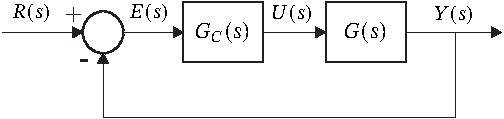
\includegraphics[scale=1]{blockdiagram.pdf}
    \fonte{Elaborada pelo autor}
\end{figure}

Caso não seja possível utilizar arquivos de imagens como \texttt{pdf}, utilize qualquer outro formato, como \texttt{jpeg}, \texttt{gif} e \texttt{bmp}. Estes formatos requerem maior tempo de processamento, mas você pode tentar aprimorar seus conteúdos com o software livre \textsf{Gimp} (\url{https://www.gimp.org/}), uma alternativa livre ao Adobe Photoshop.

Também é possível criar figuras, diagramas e gráficos utilizando comandos de pacotes disponíveis para o \LaTeX, como \textsf{TikZ}. Entretanto, tais pacotes requerem elevado tempo de processamento no Overleaf e, por isso, não foram utilizados neste documento.

Note que, de acordo com as normas da ABNT, a legenda (\texttt{caption}) das figuras e tabelas deve aparecer na parte superior. Na parte inferior deve ser informada a fonte e podem ser incluídas notas. Caso queira que a numeração e título da figura apareça na parte inferior, dentro do ambiente \texttt{figure} utilize o comando \verb|\caption| após o comando \verb|\includegraphics|. Observe também que, diferentemente da \cref{fig:blockdiag1}, a \cref{fig:blockdiag2} tem numeração e nota com a mesma largura da figura, conforme recomendado pela ABNT. A lista de todas as figuras pode ser incluída como elemento pré-textual do trabalho por meio do comando \verb|\listoffigures| no arquivo \texttt{tex} principal.

\begin{figure}[htb]
\sbox0{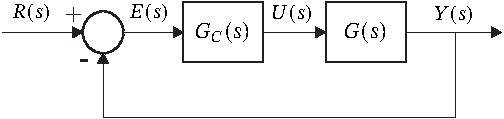
\includegraphics[scale=1]{blockdiagram.pdf}}
\centering\configurecaptions
\begin{minipage}{\wd0}
  \caption{Digrama de blocos de sistema de controle em malha fechada}
  \label{fig:blockdiag2}
  \usebox0
  \nota{Elaborada pelo autor}
\end{minipage}
\end{figure}

% ---
\subsection{Figuras em \emph{minipages}}
% ---

\emph{Minipages} são usadas para inserir textos ou outros elementos em quadros com tamanhos e posições controladas. Veja os exemplos das \cref{fig:minipage_circuito,fig:minipage_grafico}.

\begin{figure}[htb]
    \label{fig:teste}
    \centering
    \begin{minipage}[t]{0.46\textwidth}
        \centering
        \caption{Imagem da minipage}
        \label{fig:minipage_circuito}
        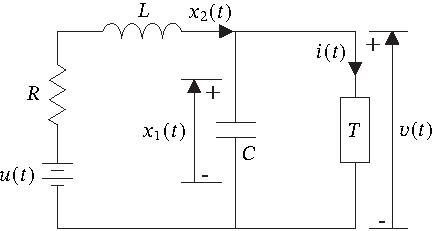
\includegraphics[scale=1]{circuito.pdf} 
        \fonte{Elaborada pelo autor}
    \end{minipage}
    \hfill
    \begin{minipage}[t]{0.52\textwidth}
        \centering
        \caption{Gráfico da minipage}
        \label{fig:minipage_grafico}
        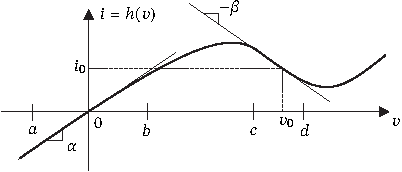
\includegraphics[scale=1.2]{diodocurva.pdf}
        \fonte{Elaborada pelo autor}
    \end{minipage}
\end{figure}

\subsection{Subfiguras}

O pacote \textsf{subfig} foi utilizado para inserir as \cref{fig:subfigura_circuito,fig:subfigura_grafico}. Subfiguras também podem ser inseridas no texto com o pacote \textsf{subcaption}.

% utiliza o pacote subfig
\begin{figure}[htb]
    \centering
    \caption{Figura com subfiguras}
    \label{fig:subfiguras}
    \subfloat[Primeira subfigura]{\label{fig:subfigura_circuito}
    \centering 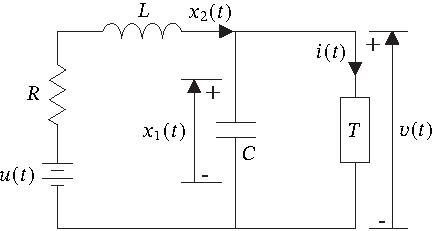
\includegraphics[scale=1]{circuito.pdf}} \hfill
    \subfloat[Segunda subfigura]{\label{fig:subfigura_grafico}
    \centering 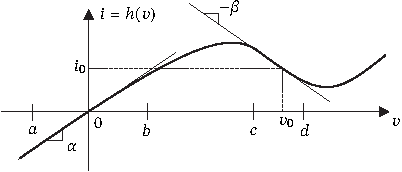
\includegraphics[scale=1.2]{diodocurva.pdf}}
    \fonte{Elaborada pelo autor}
\end{figure}

% utiliza o pacote subcaption
%\begin{figure}[htb]
%    \centering
%    \caption{Figura com subfiguras}
%    \label{fig:subfiguras}
%    \begin{subfigure}[t]{0.47\textwidth}
%        \caption{Primeira subfigura}
%        \label{fig:subfigura_circuito}
%        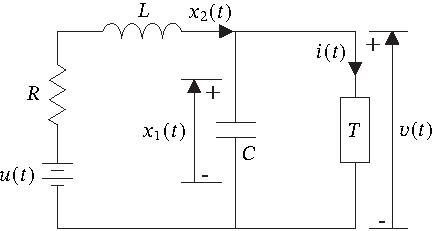
\includegraphics[scale=1]{circuito.pdf}
%    \end{subfigure}%
%    \hfill
%    \begin{subfigure}[t]{0.52\textwidth}
%        \caption{Segunda subfigura}
%        \label{fig:subfigura_grafico}
%        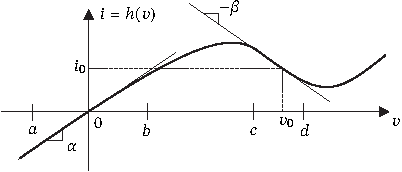
\includegraphics[scale=1.2]{diodocurva.pdf}
%    \end{subfigure}
%\end{figure}

% ---
\subsection{Figuras que usam as mesmas fontes tipográficas do documento}
% ---

Caso queira utilizar as mesmas fontes tipográficas do texto para escrever dentro de figuras, como é o caso da \cref{fig:psfrag1} (arquivo \texttt{blockdiagram.pdf}), produza uma figura como a da \cref{fig:psfrag2} e a salve no formato \texttt{eps} (arquivo \texttt{blockdiagram.eps}). Softwares como InkScape, CorelDraw ou Adobe Ilustrator podem ser utilizados para este fim.

\begin{figure}[htb]
    \centering
    \caption{Uso do pacote \textsf{psfrag}}\label{fig:psgrag}
    \subfloat[Arquivo \texttt{blockdiagram.pdf}]{\label{fig:psfrag1}
    \centering 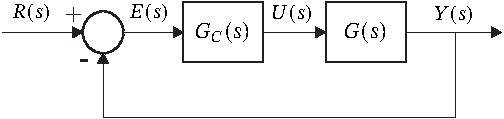
\includegraphics[scale=1]{blockdiagram.pdf}} \\
    \subfloat[Arquivo \texttt{blockdiagram.eps}]{\label{fig:psfrag2}
    \centering 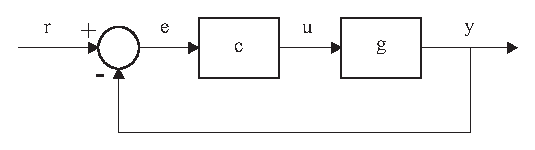
\includegraphics[scale=1]{blockdiagram.eps}}
    \fonte{Elaborada pelo autor}
\end{figure}

Crie no Overleaf um novo projeto que tenha o conteúdo do \cref{cod:tex} dentro de um arquivo \texttt{tex} nomeado, por exemplo, como \texttt{blockdiagram.tex}. No menu do Overleaf, altere o compilador de \texttt{pdfLaTeX} para \texttt{LaTeX} e defina o arquivo \texttt{blockdiagram.tex} como principal. Coloque o arquivo \texttt{blockdiagram.eps} dentro do projeto e compile. A saída gerada, corresponde à \cref{fig:psfrag1}, deve ser salva como \texttt{blockdiagram.pdf}. Este arquivo poderá ser carregado no projeto do texto do trabalho (TCC, dissertação ou tese) que você estiver escrevendo com o UnB\TeX\ (que usa o \texttt{pdfLaTeX} como compilador). Observe na \cref{fig:psfrag2} que o ``\texttt{g}'' é substituído por ``$G(s)$'' na \cref{fig:psfrag1}. Para tal, o \cref{cod:tex} utiliza o seguinte comando do pacote \textsf{psfrag}:
\begin{verbatim}
\psfrag{g}[c][c]{\footnotesize $G(s)$}
\end{verbatim}

\lstinputlisting[numbers=none,caption={\texttt{blockdiagram.tex}},label={cod:tex}]{unbtex-example/codigos/blockdiagram.tex}

O pacote \textsf{psfrag} funciona apenas com o compilador \texttt{LaTeX}, o que torna a criação de um novo projeto no Overleaf uma boa solução. Este projeto poderá ser aproveitado para gerar outras figuras do documento principal. Para mais informações sobre o pacote, consulte seu manual\footnote{Disponível em \url{https://mirrors.ctan.org/macros/latex/contrib/psfrag/pfgguide.pdf}}.

Evite o uso de figuras no formato \texttt{eps} no documento principal. Documentos que usam a classe UnB\TeX\ precisam ser compilados pelo \texttt{pdfLaTeX}, que inicialmente converte os arquivos \texttt{eps} para o formato \texttt{pdf}, exigindo maior tempo de processamento. O projeto auxiliar (\cref{cod:tex}) usa a classe \texttt{article} e admite compilador \texttt{LaTeX}, que não necessita de etapas adicionais para processar códigos que chamam arquivos \texttt{eps}.

% Capítulo de resultados
% ----------------------------------------------------------
\chapter{Ambientes do UnB\TeX}
% ----------------------------------------------------------

A classe UnB\TeX\ disponibiliza alguns ``ambientes'', ou seja, caixas de texto com formatação especial para certos tipos de elementos, que podem ser automaticamente numerados (por exemplo, \cref{def:WYSIWYG}, \cref{thm:WYSIWYG}, \cref{alg:ex}, etc.).

\section{Estilo teorema}

Criados com auxílio do pacote \textsf{mdframed}\footnote{Disponível em \url{https://mirrors.ctan.org/macros/latex/contrib/mdframed/mdframed.pdf}} e inspirados no modelo de \citeonline{Castro2019}, estão disponíveis os ambientes: \texttt{theorem}, \texttt{lemma}, \texttt{proposition}, \texttt{corollary}, \texttt{definition}, \texttt{as\-sumption}, \texttt{axiom}, \texttt{conjecture}, \texttt{property}, \texttt{example}, \texttt{exercise}, \texttt{problem}, \texttt{remark}, \texttt{proof} e \texttt{solution}. Alguns exemplos de uso são apresentados a seguir.

\begin{definition}\label{def:WYSIWYG}
O WYSIWYG (ou ``What You See Is What You Get - O que você vê é o formato final'') é um tipo de editor HTML que permite editar sua página da Web em uma visualização simplificada e sem código de aparência semelhante à do layout da página real.
\end{definition}

\begin{theorem}[Teorema LaTeX-WYSIWYG]\label{thm:WYSIWYG}
    Todo físico prefere usar código \LaTeX\ puro que qualquer editor WYSIWYG.
\end{theorem}

\begin{proof}
    Físicos gostam de equações bonitas. Editores What-You-See-Is-What-You-Get não são apropriados para fazer equações bonitas\footnote{É certo que há editores WYSIWYG baseados em \LaTeX, mas eles não nos dão o mesmo nível de controle.}. Logo, se algum físico preferisse usar um editor WYSIWYG no lugar de \LaTeX, não seria muito inteligente. Como todo físico é inteligente, o teorema está demonstrado \textit{ad absurdum}.
\end{proof}

\begin{proposition}\label{prop:WYSIWYG}
    \LaTeX\ produz equações mais bonitas que qualquer editor WYSIWYG.
\end{proposition}

\begin{lemma}
    Teste.
\end{lemma}

\begin{corollary}
    Teste.
\end{corollary}

\begin{remark}
    \LaTeX\ produz equações mais bonitas que qualquer editor WYSIWYG.
\end{remark}

\begin{exercise}\label{exc:in}
    Explique como Isaac Newton usaria cada um dos pacotes seguintes, se vivesse no tempo presente:
    \begin{enumerate}[label=(\alph*)]
        \item Metapost
        \item TikZ
        \item PGFPlots
        \item PSTricks
    \end{enumerate}
\end{exercise}

%\begin{example}\label{exp:ae}
%    Einstein usaria um editor WYSIWYG ou \LaTeX? \\
%    Einstein era físico. Portanto, usando o teorema LaTeX-WYSIWYG, concluímos que ele usaria \LaTeX.
%\end{example}

\section{Pseudocódigos}

O \cref{alg:ex} é um exemplo de pseudocódigo, inserido com auxílio do pacote \textsf{algorithm2e}. Mais opções de uso (e de comandos) podem ser encontradas em seu manual\footnote{Disponível em \url{https://mirrors.ctan.org/macros/latex/contrib/algorithm2e/doc/algorithm2e.pdf}}.

\begin{algorithm}[htb]
\caption{Exemplo de pseudocódigo}\label{alg:ex}
\KwData{$n \geq 0$}
\KwResult{$y = x^n$}
$y \gets 1$\;
$X \gets x$\;
$N \gets n$\;
%\While{$N \neq 0$}{
\While(\tcc*[f]{Isso é um comentário}){$N \neq 0$}{
  \eIf{$N$ for par}{
    $X \gets X \times X$\;
    $N \gets \frac{N}{2}$ \tcc*[r]{Isso é outro comentário}
  }{\If{$N$ for ímpar}{
      $y \gets y \times X$\;
      $N \gets N - 1$\;
    }
  }
}
\end{algorithm}

A lista com todos os algoritmos é um elemento pré-textual não obrigatório de trabalhos acadêmicos e pode ser gerada e incluída utilizando-se o comando \verb|\listofalgorithms| no arquivo \texttt{tex} principal.

\section{Códigos-fonte}

O \cref{cod:exemplo} é um exemplo de código-fonte, inserido com auxílio do pacote \textsf{listings}. Para mais exemplos e comandos, confira o \cref{apd:cdg} e o manual do pacote\footnote{Disponível em \url{https://mirrors.ctan.org/macros/latex/contrib/listings/listings.pdf}}. A lista com todos os códigos-fonte é um elemento pré-textual não obrigatório de trabalhos acadêmicos e pode ser gerada e incluída utilizando-se o comando \verb|\lstlistoflistings| no arquivo \texttt{tex} principal.

\begin{lstlisting}[float=htb,caption={Exemplo de código-fonte},label={cod:exemplo}]
/**
* MSO: ativa o servo cujo eixo eh descrito
* por drive_axis; informacoes de controle
* sao gravadas em MSO_1
*/
  MSO(drive_axis,MSO_1);
/* Atribui o valor 0.0 ao primeiro elemento do array speed */
  speed[0] := 0.0; 
/* Atribui 1 para dataInitialized */
  dataInitialized := 1;
\end{lstlisting}

% Capítulo de conclusões
% ----------------------------------------------------------
\chapter{Conclusões}
% ----------------------------------------------------------

Você deve começar a editar o seu TCC/Dissertação/Tese agora mesmo!

% ------------------------------------------------------------------------
% ELEMENTOS PÓS-TEXTUAIS
% ------------------------------------------------------------------------
\postextual
% ------------------------------------------------------------------------

% ---
% Referências bibliográficas
% ---
% Arquivo com as referências bibliográficas
\bibhang{2.2em} % Recuo da margem esquerda da lista de referências
\bibliography{unbtex-example/referencias} % O estilo de citação é selecionado automaticamente
% ---

% ---
% Apêndices
% ---
\begin{apendicesenv}

% Imprime uma página indicando o início dos apêndices
\partapendices

% ----------------------------------------------------------
\chapter{Citações}\label{apd:cit}
% ----------------------------------------------------------

A classe UnB\TeX\ usa o pacote \texttt{abntex2cite} para formatar as referências bibliográficas conforme as regras da ABNT. O arquivo \texttt{referencias.bib}, utilizado neste documento, contém várias entradas de bibliografia, que podem ser utilizadas como modelos para incluir outras entradas e citá-las por meio dos seguintes comandos:
\begin{verbatim}
\cite{nome_da_entrada}
\citeonline{nome_da_entrada}
\citeauthoronline{nome_da_entrada}
\citeyear{nome_da_entrada}
\end{verbatim}

Considere, por exemplo, a entrada para referência do tipo manual (\texttt{@manual}) contida no arquivo \texttt{referencias.bib}:
\begin{verbatim}
@manual{memoir,
    address = {Normandy Park, WA},
    author = {Peter Wilson and Lars Madsen},
    organization = {The Herries Press},
    title = {The Memoir Class for Configurable Typesetting -- User Guide},
    url = {https://mirrors.ctan.org/macros/latex/contrib/memoir/memman.pdf},
    year = {2024}}
\end{verbatim}

Utilizando-se o comando \verb|\cite{memoir}| no arquivo \texttt{tex} correspondente a este parágrafo do \cref{apd:cit}, o resultado gerado é \cite{memoir}. Para o comando \verb|\citeonline{memoir}|, o resultado gerado é \citeonline{memoir}. Note que se o estilo de citação utilizado for o numérico, os comandos \verb|\cite| e \verb|\citeonline| geram o mesmo resultado, conforme mencionado na \cref{sec:referencias}.

Os comandos \verb|\citeauthoronline| e \verb|\citeyear|, tanto no estilo autor-ano como no estilo numérico, apresentam separadamente no texto o nome dos autores e o ano da publicação. Por exemplo, podemos escrever:

\begin{mdframed}[style=plainSty,innertopmargin=8pt] % verde
Em \citeyear{memoir}, os autores \citeauthoronline{memoir} publicaram o manual da versão v3.8.2 do pacote \textsf{memoir}.
\end{mdframed}

No arquivo \texttt{bib}, cada entrada de referência bibliográfica possuiu campos cujo preenchimento pode ser obrigatório ou opcional, a depender de seu tipo. No campo \texttt{author}, caso haja mais de um autor, seus nomes devem ser separados por \texttt{and}. Campos como \texttt{address}, \texttt{publisher} e \texttt{year} não preenchidos, podem gerar na lista de referências, respectivamente, as expressões abreviadas [\emph{s.l.}], [\emph{s.n.}] e [\emph{s.d.}] para indicar que são indeterminados. Recomenda-se o uso de programas gratuitos, como o JabRef\footnote{Disponível em: \url{https://www.jabref.org/}}, para auxiliar o preenchimento e gerenciamento de arquivos \texttt{bib}.

No arquivo \texttt{referencias.bib}, além da entrada para referência do tipo manual (como no exemplo dado), há também entradas para referências do tipo artigo de periódico \cite{greenwade93}, artigo de conferência \cite{martin1997}, livro \cite{schaum1956}, capítulo de livro \cite{bates2010}, monografia \cite{morgado1990}, dissertação de mestrado \cite{macedo2005}, tese de doutorado \cite{guizzardi2005}, relatório técnico \cite{KrueBansBierDaziRash20}, dentre outras. Muitos outros exemplos podem ser encontrados em \cite{abntex2cite}.

Note que de acordo com as normas da ABNT, é obrigatório informar data para cada referência bibliográfica. Caso a data não seja identificada na referência, deve-se informar uma data aproximada entre colchetes, conforme situações ilustradas a seguir:

\begin{alineas}
    \item um ano ou outro: [2007 ou 2008]
    \item data provável: [2008?]
    \item data certa não indicada no item: [2008]
    \item use intervalos menores de 20 anos: [entre 1999 e 2008]
    \item data aproximada: [ca. 2000]
    \item década certa: [200-]
    \item década provável: [200-?]
    \item século certo: [20--]
    \item século provável: [20--?]
\end{alineas}

Em \citeonline{Metodista}, por exemplo, o ano provável é indicado por \citeyear{Metodista}. No arquivo \texttt{bib}, a entrada correspondente a esta referência tem o campo \texttt{year} declarado como:
\begin{verbatim}
    year = {$\lbrack$2015?$\rbrack$}
\end{verbatim}
Para não ocorrer erro na compilação do documento, deve-se utilizar os comandos \verb|$\lbrack$| e \verb|$\rbrack$| para os colchetes ``['' e ``]'', respectivamente.

% ----------------------------------------------------------
\chapter{Tabelas longas e rotacionadas}\label{apd:tabs}
% ----------------------------------------------------------

A \cref{tab:dscf} é um exemplo de tabela longa, que ocupa mais de uma página, construída com o ambiente \texttt{longtable} do pacote com mesmo nome (para mais informações sobre o pacote, consulte seu manual\footnote{Disponível em \url{https://mirrors.ctan.org/macros/latex/required/tools/longtable.pdf}}). Para quadros longos, utilize o ambiente \texttt{longquadro}, disponibilizado na classe UnB\TeX. 

A \cref{tab:rot} foi construída com o ambiente \texttt{landscape} do pacote \textsf{lscape}. Para rotacionar, além da tabela, também a página do arquivo \texttt{pdf}, utilize o pacote \textsf{pdflscape}\footnote{Disponível em \url{http://mirrors.ctan.org/macros/latex/contrib/pdflscape/pdflscape.pdf}}. De forma análoga, os pacotes mencionados para rotacionar tabelas, podem rotacionar figuras.

\begin{longtable}{L{2.5cm}C{2.5cm}C{1cm}C{1.5cm}C{1cm}C{1.5cm}C{1cm}C{1.5cm}}
%\begin{longquadro}{L{2.5cm}C{2.5cm}C{1cm}C{1.5cm}C{1cm}C{1.5cm}C{1cm}C{1.5cm}}
% Cabeçalho no início da tabela
\caption{Tabela longa}
\label{tab:dscf} \\
\toprule
\multirow{3}{*}{\bfseries Variable} & 
\multirow{3}{*}{\parbox{2.5cm}{\centering\bfseries Proportions in Sample (\%)}} & 
\multicolumn{6}{c}{\bfseries Proportions by Subtype (\%)} \\
\cmidrule(lr){3-8}
& &
\multicolumn{2}{c}{\bfseries Graduated} & \multicolumn{2}{C{3cm}}{\bfseries Academically Excluded} & 
\multicolumn{2}{c}{\bfseries Censored} \\
\midrule
\endfirsthead
% Cabeçalho da continuação da tabela no topo da página seguinte
\caption[]{Tabela longa (continuação)} \\ \toprule
\multirow{3}{*}{\bfseries Variable} & 
\multirow{3}{*}{\parbox{2.5cm}{\centering\bfseries Proportions in Sample (\%)}} & 
\multicolumn{6}{c}{\bfseries Proportions by Subtypes (\%)} \\
\cmidrule(lr){3-8}
& &
\multicolumn{2}{c}{\bfseries Graduated} & \multicolumn{2}{C{3cm}}{\bfseries Academically Excluded} & 
\multicolumn{2}{c}{\bfseries Censored} \\
\midrule
\endhead
\hline
\multicolumn{8}{r}{(Continua)}\\
\endfoot
\bottomrule
\endlastfoot
\bfseries Total & 100.0 & 50.1 & (45.8) & 7.5 & (14.9) & 42.4 & (39.3) \\
\addlinespace
\bfseries Gender \\
Male   & 52.4 & 49.6 & (44.3) & 8.7 & (17.3) & 41.7 & (38.5) \\
Female & 47.6 & 50.7 & (48.0) & 6.2 & (11.5) & 43.1 & (40.5) \\
\addlinespace
\bfseries Race \\
White & 40.3 & 59.8 & (58.7) & 3.0 & (4.6) & 37.2 & (36.7) \\
Black & 32.4 & 38.7 & (32.5) & 13.1 & (26.3) & 48.2 & (41.2) \\
Coloured & 13.0 & 49.8 & (44.5) & 7.4 & (16.1) & 42.8 & (39.5) \\
Indian/Asian & 14.3 & 48.9 & (44.6) & 7.9 & (13.3) & 43.3 & (42.1) \\
\addlinespace
\bfseries Financial Aid \\
Ineligible for Financial Aid & 82.3 & 52.1 & (48.7) & 5.5 & (10.6) & 42.4 & (40.7) \\
Eligible for Financial Aid & 17.7 & 40.7 & (35.2) & 17.2 & (30.3) & 42.1 & (34.5) \\
\addlinespace
\bfseries Programme \\
Mainstream & 76.9 & 55.4 & (51.3) & 5.7 & (10.8) & 38.9 & (37.9) \\
Academic Development & 23.1 & 32.5 & (27.1) & 13.7 & (28.7) & 53.8 & (44.2) \\
\addlinespace
\bfseries English Home Language \\
Yes & 69.3 & 55.1 & (52.8) & 4.9 & (8.6) & 39.9 & (38.6) \\
No & 30.7 & 38.8 & (32.8) & 13.4 & (26.6) & 47.8 & (40.6) \\
\addlinespace
\bfseries School Quintile \\
1 & 0.8 & 34.6 & (26.1) & 30.8 & (42.6) & 34.6 & (31.3) \\
2 & 1.6 & 30.2 & (28.1) & 16.0 & (35.1) & 53.8 & (36.8) \\
3 & 5.0 & 32.0 & (27.7) & 17.5 & (35.3) & 50.5 & (37.0) \\
4 & 4.1 & 37.7 & (29.5) & 17.7 & (32.0) & 44.5 & (38.5) \\
5 & 45.4 & 52.0 & (49.2) & 6.9 & (12.0) & 41.1 & (38.9) \\
Independent  & 43.1 & 52.5 & (50.4) & 5.3 & (8.6) & 42.2 & (41.0) \\
\addlinespace
{\bfseries Province} \\
Western Cape & 40.0 & 55.1 & (51.3) &5.9 & (11.6) &39.0 & (37.0) \\
Non-Western Cape & 59.9 & 46.8 & (41.9) & 8.6 & (17.2) & 44.6 & (41.0) \\
\addlinespace
{\bfseries Year of First Registration} \\
{2006} & 11.6  & 87.8 & (79.9) & 11.3 & (18.9) & 0.9 & (1.2) \\
{2007} & 11.9 & 88.2 & (79.4) & 10.1 & (19.2)   & 1.7 & (1.4) \\
{2008} & 12.6 & 87.1 & (76.7) & 10.3 & (20.3) & 2.6 & (3.0) \\
{2009} & 11.9 & 80.9 & (64.9) & 9.7 & (24.9) & 9.4 & (10.2) \\
{2010} & 11.1 & 62.6 & (57.5) & 6.4 & (12.7) & 31.1 & (29.8) \\
{2011} & 11.7 & 15.8 & (15.3) & 7.2 & (12.8) & 77.0 & (71.9) \\
{2012} & 14.1 & 0.0 & (0.0)  & 5.4 & (7.5) & 94.6 & (92.5) \\
{2013} & 15.1 & 0.0 & (0.0) & 1.7 & (3.0) & 98.3 & (97.0) \\
%\end{longquadro}
\end{longtable}

\afterpage{ % Evita quebra de página ao inserir tabela rotacionada
\begin{landscape} % Rotaciona a tabela
\begin{table}%
\centering\small
\caption{Tabela rotacionada}\label{tab:rot}
\setlength\tabcolsep{3pt} % define o espaçamento entre colunas
\begin{tabular}{@{}L{1.1cm}L{1.6cm}L{1.6cm}L{1.6cm}L{1.6cm}L{1.6cm}L{1.6cm}L{1.6cm}L{1.6cm}L{1.6cm}L{1.6cm}L{1.6cm}L{1.6cm}@{}} % @{} elimina o espaço nas bordas laterais
\toprule
Sv,ieq & 000436xa & 000594xa & 001715xa & 001932ya & 006040ya & 006263xa & 007162ya & 007257ya & IT0605ya & IT0790xa & emiliaeo-retro & emilians-retro \\ \midrule
0.4 & 2.447  & 2.177  & 2.304  & 4.921  & 4.298  & 2.121  & 3.928  & 3.478  & 3.462  & 1.751  & 0.875  & 0.525 \\
0.8 & 4.894  & 4.354  & 4.609  & 9.843  & 8.597  & 4.241  & 7.857  & 6.957  & 6.924  & 3.502  & 1.750  & 1.049 \\
1.2 & 7.341  & 6.530  & 6.913  & 14.764 & 12.895 & 6.362  & 11.785 & 10.435 & 10.386 & 5.252  & 2.625  & 1.574 \\
1.6 & 9.789  & 8.707  & 9.218  & 19.686 & 17.194 & 8.482  & 15.713 & 13.914 & 13.848 & 7.003  & 3.500  & 2.099 \\
2   & 12.236 & 10.884 & 11.522 & 24.607 & 21.492 & 10.603 & 19.642 & 17.392 & 17.310 & 8.754  & 4.375  & 2.624 \\
2.4 & 14.683 & 13.061 & 13.827 & 29.529 & 25.791 & 12.723 & 23.570 & 20.871 & 20.772 & 10.505 & 5.250  & 3.148 \\
2.8 & 17.130 & 15.237 & 16.131 & 34.450 & 30.089 & 14.844 & 27.498 & 24.349 & 24.234 & 12.256 & 6.125  & 3.673 \\
3.2 & 19.577 & 17.414 & 18.435 & 39.372 & 34.388 & 16.965 & 31.427 & 27.828 & 27.697 & 14.006 & 7.000  & 4.198 \\
3.6 & 22.024 & 19.591 & 20.740 & 44.293 & 38.686 & 19.085 & 35.355 & 31.306 & 31.159 & 15.757 & 7.875  & 4.723 \\
4   & 24.471 & 21.768 & 23.044 & 49.215 & 42.984 & 21.206 & 39.283 & 34.784 & 34.621 & 17.508 & 8.750  & 5.247 \\
4.4 & 26.919 & 23.945 & 25.349 & 54.136 & 47.283 & 23.326 & 43.212 & 38.263 & 38.083 & 19.259 & 9.625  & 5.772 \\
4.8 & 29.366 & 26.121 & 27.653 & 59.058 & 51.581 & 25.447 & 47.140 & 41.741 & 41.545 & 21.009 & 10.500 & 6.297 \\
5.2 & 31.813 & 28.298 & 29.957 & 63.979 & 55.880 & 27.567 & 51.068 & 45.220 & 45.007 & 22.760 & 11.375 & 6.821 \\
5.6 & 34.260 & 30.475 & 32.262 & 68.900 & 60.178 & 29.688 & 54.996 & 48.698 & 48.469 & 24.511 & 12.250 & 7.346 \\
6   & 36.707 & 32.652 & 34.566 & 73.822 & 64.477 & 31.809 & 58.925 & 52.177 & 51.931 & 26.262 & 13.125 & 7.871 \\ \bottomrule 
\end{tabular}
\end{table}%
\end{landscape}
}

% ----------------------------------------------------------
\chapter{Códigos de programação}\label{apd:cdg}
% ----------------------------------------------------------

\section{Projeto do controlador por realimentação de estados}
\lstinputlisting[language=Matlab,caption={Código de Matlab},label={cod:matlab}]{unbtex-example/codigos/controle.m}

\section{Exemplo de teste em malha fechada com entrada rampa}
\lstinputlisting[language=Python,caption={Código de Python},label={cod:python}]{unbtex-example/codigos/controleSmithPredictor.py}

\section{Redução modal}
\lstinputlisting[language=Julia,caption={Código de Julia},label={cod:julia}]{unbtex-example/codigos/ModalReduction.jl}

\end{apendicesenv}
% ---

% ---
% Anexos
% ---
\begin{anexosenv}

% Imprime uma página indicando o início dos anexos
\partanexos

% ----------------------------------------------------------
\chapter{Paleta de cores da UnB}\label{anx:coresunb}
% ----------------------------------------------------------

A paleta de cores da UnB, disponível na \cpageref{marcaunb.1} a seguir, foi extraída do \emph{manual de identidade visual}\footnote{Disponível em \url{http://marca.unb.br}} da Universidade.

Note que, de acordo com a ABNT, a principal diferença entre anexo e apêndice é que os apêndices são textos criados pelo próprio autor para complementar sua argumentação, enquanto os anexos são documentos criados por terceiros, e usados pelo autor.

\cleardoublepage

\newcounter{includepdfpage} % para referenciar no texto páginas pdf incluídas

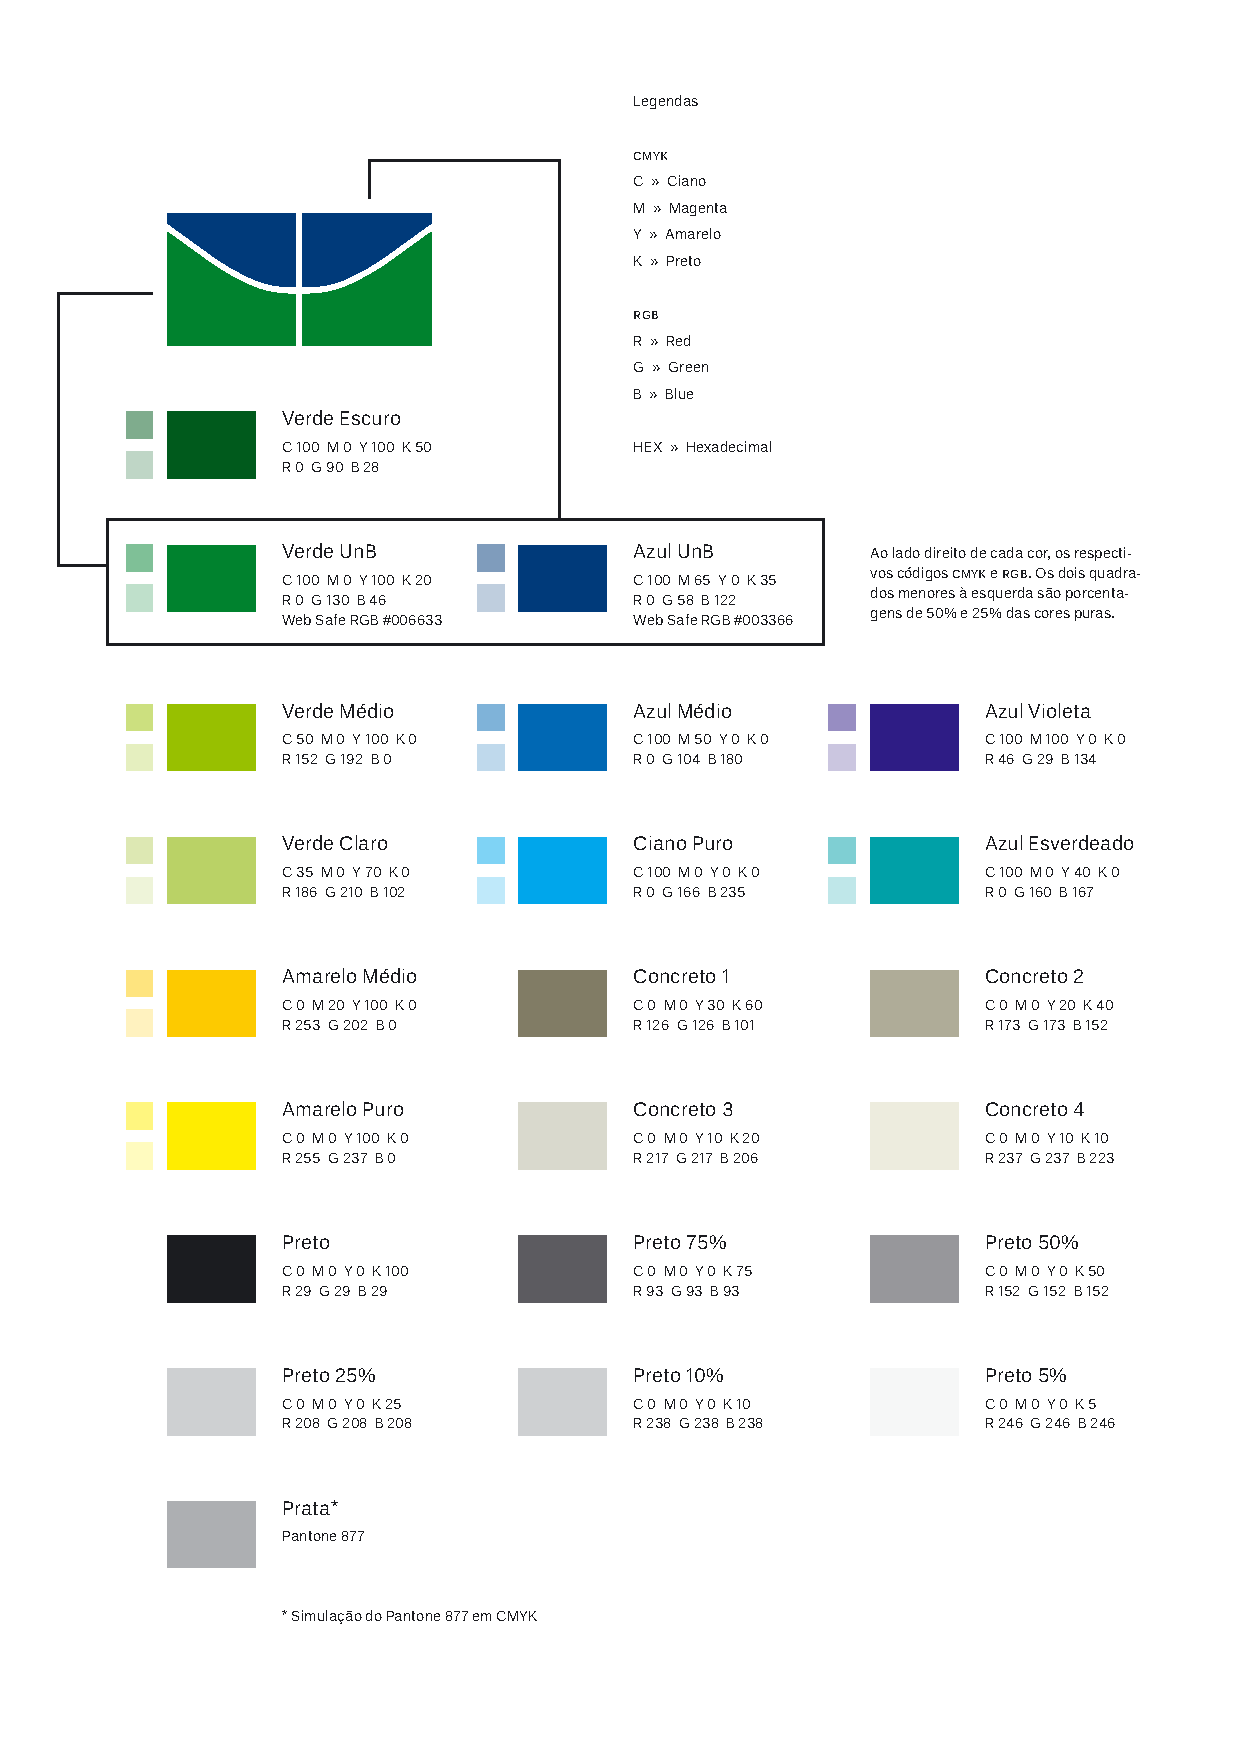
\includepdf[
    pages=-, % intervalo das páginas do arquivo pdf que serão incluídas
    scale=1, % controla o tamanho da página inserida
    pagecommand={\thispagestyle{plain} % imprime o número da página
    \refstepcounter{includepdfpage} % conta a página incluída
    \label{marcaunb.\theincludepdfpage} % marcaunb.n, n número da página
    },
    ]{unbtex-example/figuras/coresunb}

\cleardoublepage

\end{anexosenv}
% ---

\end{document}